\documentclass[12pt,a4paper]{article}

\title{JSP3: Eval}
\author{Zuzana Smetanová\\ 
(\href{https://github.com/zsmetanova}{zsmetanova})\\
\href{mailto:smetzu00@upol.cz}{smetzu00@upol.cz}}

\usepackage[dvipsnames]{xcolor}
\usepackage[colorlinks=true]{hyperref}
\hypersetup{
    citecolor=OliveGreen, % a very dark green
    linkcolor=NavyBlue,
    urlcolor=NavyBlue
  }
\usepackage{url}
\usepackage{graphicx} % Required for inserting images
\usepackage{booktabs}
\usepackage{float}

\usepackage{pgfplots}
\pgfplotsset{compat=1.18}

\begin{document}
\maketitle

\section{Introduction}
\label{sec:introduction}
This report evaluates the performance of the model \texttt{spec\_qwen3:4b.json} using the gold standard dataset \texttt{spec\_human.json}. The goal is to compare the model predictions with human annotations and measure how accurate the model is.

We focus on several aspects of evaluation. First, we calculate the overall accuracy of the model. Then, we analyze the results by different POS tag types and look at the most common errors. We also use WordNet to measure semantic similarity between gold and predicted synsets and compute near-miss scores. This helps us understand whether the model predictions are completely wrong or only slightly different in meaning.

\section{Background}
\label{sec:background}
For semantic evaluation, we use WordNet through the NLTK library. WordNet is a lexical database of English words, where words are grouped into sets called synsets. Each synset represents one meaning of a word.

WordNet also stores relations between synsets, such as synonymy and hypernymy. These relations allow us to measure how close two meanings are. In this evaluation, WordNet is used to check whether the model predicts a synset that is semantically close to the correct one.

\subsection*{Resources}
\label{sec:resources}

The WordNet corpus is provided by the NLTK library. It allows us to compute semantic similarity between synsets. In our evaluation, we use the Wu-Palmer similarity measure, which compares synsets based on their position in the WordNet hierarchy.

\section{Approach}
\label{sec:approach}
The evaluation was located in the file \texttt{eval.py}. The input files are loaded using \texttt{argparse}. For each token, the model prediction is compared with the gold standard annotation.

We first compute the total accuracy. Then, we calculate accuracy for each POS tag type. Confusion matrices are created for POS tags and for synsets to analyze common mistakes. Precision, recall, and F1 scores are computed in both macro and micro variants.

To evaluate near-miss errors, we use WordNet from the NLTK library. Semantic similarity between synsets is computed using the Wu-Palmer similarity (\texttt{wup\_similarity()}). We also calculate accuracy without the POS tag "x", because this tag causes many errors and strongly affects the final results.

\section{Results}
\label{sec:results}
\subsection*{Accuracy}
\begin{itemize}
    \item Total accuracy: 57.87\%
    \item Accuracy without "x" POS: 88.05\% (5616/6378)
\end{itemize}

\subsection*{Breakdown by Tag}
\begin{table}[H]
\centering
\caption{Break down results by tag type}
\label{tab:tag-results}
\begin{tabular}{l c l}
\toprule
Tag & Correct & Count \\
\midrule
a & 75.60\% & (914/1209)\\
dat:year & 0.00\% & (0/1)\\
loc & 94.12\% & (16/17)\\
n & 64.18\% & (1851/2884)\\
num  & 100.00\% & (3/3)\\
org & 50.00\% & (1/2)\\
oth & 50.00\% & (1/2)\\
per & 95.92\% & (47/49)\\
r & 75.26\% & (569/756)\\
v & 60.62\% & (882/1455)\\
x & 28.13\% & (561/1994)\\
\bottomrule
\end{tabular}
\end{table}

\subsection*{Confusion Matrix POS}
\begin{table}[H]
\centering
\caption{Confusion matrix POS}
\resizebox{\textwidth}{!}{
\begin{tabular}{lcccccccccccccccccc}
\hline
POS & MISSING & a & dat & dat:year & e & loc & n & num & org & oth & per & r & v & w & x & year & z \\
\hline
MISSING & \textcolor{green}{0} & \textcolor{red}{1} & 0 & 0 & 0 & 0 & 0 & 0 & 0 & 0 & 0 & 0 & 0 & 0 & 0 & 0 & 0 \\
a & \textcolor{red}{31} & \textcolor{green}{1085} & \textcolor{red}{1} & 0 & 0 & 0 & \textcolor{red}{28} & \textcolor{red}{24} & 0 & \textcolor{red}{2} & 0 & \textcolor{red}{52} & \textcolor{red}{5} & \textcolor{red}{1} & \textcolor{red}{11} & 0 & 0 \\
dat & 0 & 0 & \textcolor{green}{0} & 0 & 0 & 0 & 0 & 0 & 0 & 0 & 0 & 0 & 0 & 0 & 0 & 0 & 0 \\
dat:year & 0 & 0 & 0 & \textcolor{green}{0} & 0 & 0 & 0 & 0 & 0 & 0 & 0 & 0 & 0 & 0 & 0 & \textcolor{red}{1} & 0 \\
e & 0 & 0 & 0 & 0 & \textcolor{green}{0} & 0 & 0 & 0 & 0 & 0 & 0 & 0 & 0 & 0 & 0 & 0 & 0 \\
loc & 0 & 0 & 0 & 0 & 0 & \textcolor{green}{16} & 0 & 0 & \textcolor{red}{1} & 0 & 0 & 0 & 0 & 0 & 0 & 0 & 0 \\
n & \textcolor{red}{51} & \textcolor{red}{77} & \textcolor{red}{17} & 0 & 0 & \textcolor{red}{31} & \textcolor{green}{2390} & \textcolor{red}{12} & 0 & \textcolor{red}{10} & \textcolor{red}{27} & \textcolor{red}{33} & \textcolor{red}{59} & \textcolor{red}{12} & \textcolor{red}{214} & \textcolor{red}{2} & 0 \\
num & 0 & 0 & 0 & 0 & 0 & 0 & 0 & \textcolor{green}{3} & 0 & 0 & 0 & 0 & 0 & 0 & 0 & 0 & 0 \\
org & 0 & 0 & 0 & 0 & 0 & 0 & \textcolor{red}{1} & 0 & \textcolor{green}{1} & 0 & 0 & 0 & 0 & 0 & 0 & 0 & 0 \\
oth & 0 & \textcolor{red}{1} & 0 & 0 & 0 & 0 & 0 & 0 & 0 & \textcolor{green}{1} & 0 & 0 & 0 & 0 & 0 & 0 & 0 \\
per & 0 & 0 & 0 & 0 & 0 & 0 & \textcolor{red}{2} & 0 & 0 & 0 & \textcolor{green}{47} & 0 & 0 & 0 & 0 & 0 & 0 \\
r & \textcolor{red}{7} & \textcolor{red}{15} & \textcolor{red}{8} & 0 & 0 & 0 & \textcolor{red}{13} & \textcolor{red}{1} & 0 & 0 & 0 & \textcolor{green}{679} & \textcolor{red}{2} & \textcolor{red}{1} & \textcolor{red}{37} & 0 & 0 \\
v & \textcolor{red}{50} & \textcolor{red}{2} & 0 & 0 & 0 & \textcolor{red}{1} & \textcolor{red}{37} & 0 & 0 & 0 & 0 & \textcolor{red}{4} & \textcolor{green}{1394} & \textcolor{red}{6} & \textcolor{red}{11} & 0 & 0 \\
w & 0 & 0 & 0 & 0 & 0 & 0 & 0 & 0 & 0 & 0 & 0 & 0 & 0 & \textcolor{green}{0} & 0 & 0 & 0 \\
x & \textcolor{red}{37} & \textcolor{red}{329} & \textcolor{red}{6} & \textcolor{red}{2} & \textcolor{red}{3} & \textcolor{red}{2} & \textcolor{red}{81} & \textcolor{red}{5} & 0 & \textcolor{red}{1} & \textcolor{red}{1} & \textcolor{red}{282} & \textcolor{red}{505} & \textcolor{red}{35} & \textcolor{green}{657} & \textcolor{red}{1} & \textcolor{red}{86} \\
year & 0 & 0 & 0 & 0 & 0 & 0 & 0 & 0 & 0 & 0 & 0 & 0 & 0 & 0 & 0 & \textcolor{green}{0} & 0 \\
z & 0 & 0 & 0 & 0 & 0 & 0 & 0 & 0 & 0 & 0 & 0 & 0 & 0 & 0 & 0 & 0 & \textcolor{green}{0} \\
\hline
\end{tabular}
}

\subsection*{Top Synset Confusions}
\begin{table}[H]
\centering
\caption{Top synset confusions}
\begin{tabular}{lcc}
\toprule
Gold & Model & Count\\
\midrule
be.v.01 & exist.v.01 & 21\\
miss.n.03 & girl.n.01 & 17\\
be.v.05 & be.v.01 & 17\\
state.v.01 & say.v.08 &13\\
hand.n.13 & hand.n.01 &11\\
exist.v.01 & be.v.01 & 11\\
be.v.02 & be.v.01 & 9\\
be.v.01 & be.v.05 & 9\\
however.r.02 & however.r.01 & 7\\
window.n.01 & window.n.07 & 6\\
\bottomrule
\end{tabular}
\end{table}

\end{table}

\subsection*{F-score Summary}
\begin{table}[H]
\centering
\caption{F1 Summary}
\begin{tabular}{lccc}
\toprule
Type & Precision & Recall & F1\\
\midrule
Macro & 0.482 & 0.703 & 0.513\\
Micro & 0.734 & 0.73 & 0.734\\
\bottomrule
\end{tabular}
\end{table}

\subsection*{Error Types}
\begin{table}[H]
\centering
\caption{Type of error}
\begin{tabular}{lc}
\toprule
Type & Count\\
\midrule
mismatch\_pos & 1977\\
generalized\_tag & 5\\
mismatch\_offset & 1127\\
coarse\_tag & 117\\
missing\_target\_tag & 176\\
unknown\_tag & 301\\
missing\_gold\_tag & 1\\
\bottomrule
\end{tabular}
\end{table}


\subsection*{Near-miss Score}
\begin{table}[H]
\centering
\caption{Near-miss error examples}
\begin{tabular}{lcc}
\toprule
Gold & Model & Near-miss\\
\midrule
summon.v.02 & call.v.05 & 0.947\\
cat.n.01 & big\_cat.n.01 & 0.929\\
request.v.01 & invite.v.07 & 0.909\\
costume.n.04 & costume.n.01 & 0.900\\
edge.n.01 & boundary\_line.n.01 & 0.875\\
\bottomrule
\end{tabular}
\end{table}

\subsection*{Near-miss Histogram}
\begin{figure}[H]
\centering
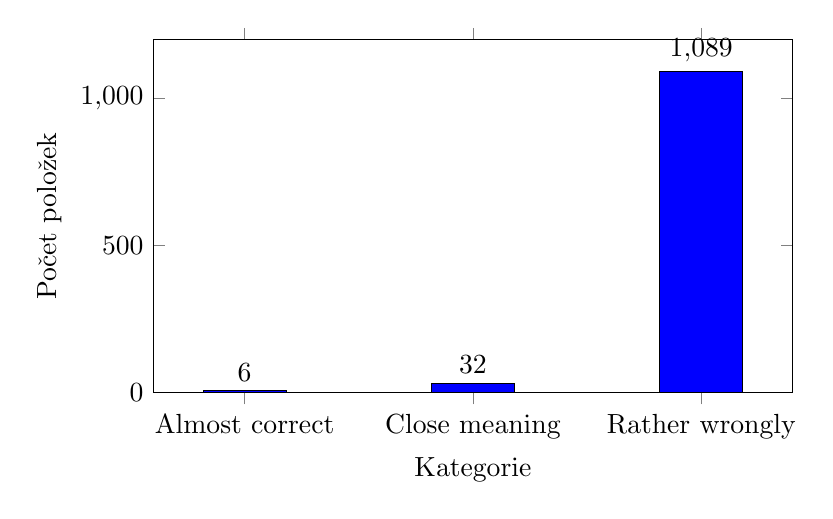
\begin{tikzpicture}
\begin{axis}[
    ybar,
    bar width=30pt,
    width=0.8\textwidth,
    height=0.5\textwidth,
    xlabel={Kategorie},
    ylabel={Počet položek},
    symbolic x coords={Almost correct, Close meaning, Rather wrongly},
    xtick=data,
    nodes near coords,
    enlarge x limits=0.2,
    ymin=0,
]
\addplot[fill=blue] coordinates {
    (Almost correct,6)
    (Close meaning,32)
    (Rather wrongly,1089)
};
\end{axis}
\end{tikzpicture}
\caption{Histogram kvality Near-miss predikcí}
\end{figure}

\textbf{Average near-miss score:} 0.424\\  
\textbf{Near-miss weighted F1:} 0.381

\section{Discussion}
\label{sec:discussion}
Our evaluation shows that the model has overall accuracy of 57.87\%. When we ignore the problematic POS tag "x", the accuracy increases to 88.05\%. This means the model works well for normal and clear tokens, but unknown or unclear tokens make the performance worse.

Looking at tag results, the model is very good at numbers ("num"), person names ("per"), and locations ("loc"). It is worse at nouns ("n") and verbs ("v") and almost fails on very rare tags like `dat:year`. This is probably because there are fewer examples of these tags in the dataset.

The confusion matrix and synset analysis show that the model often predicts similar but not exact meanings. Near-miss score (average 0.424) shows many mistakes are close in meaning. So the model understands the context, but not always the exact sense.

The main types of errors are POS mismatch and offset mismatch. This shows problems with tokenization or alignment with the gold data. Future work can focus on:
\begin{itemize}
    \item Improving the handling of unknown POS tags ("x") and rare tags.
    \item Teaching the model to better distinguish similar meanings in synsets.
\end{itemize}

\section{Conclusions}
\label{sec:conclusions}
In this report, we evaluated the model \texttt{spec\_qwen3:4b.json} on the dataset \texttt{spec\_human.json}. The overall accuracy is 57.87\%, and without the "x" tag it is 88.05\%. The model works well on common and clear tokens, but rare and unclear tags are harder to predict.

The confusion matrix and near-miss scores show that many mistakes are semantically close. Future improvements can include better handling of rare tags, better distinction of similar meanings.
\end{document}
